\documentclass[tikz]{standalone}
\usepackage{tikz}

\usetikzlibrary{positioning}
\usetikzlibrary{fit}
\usetikzlibrary{shapes}
\usetikzlibrary{arrows}

\tikzstyle{X} = [circle,fill=white,draw=black]
% Observed node
\tikzstyle{Y} = [X,fill=gray!25]
\tikzset{>={triangle 45}}

\begin{document}

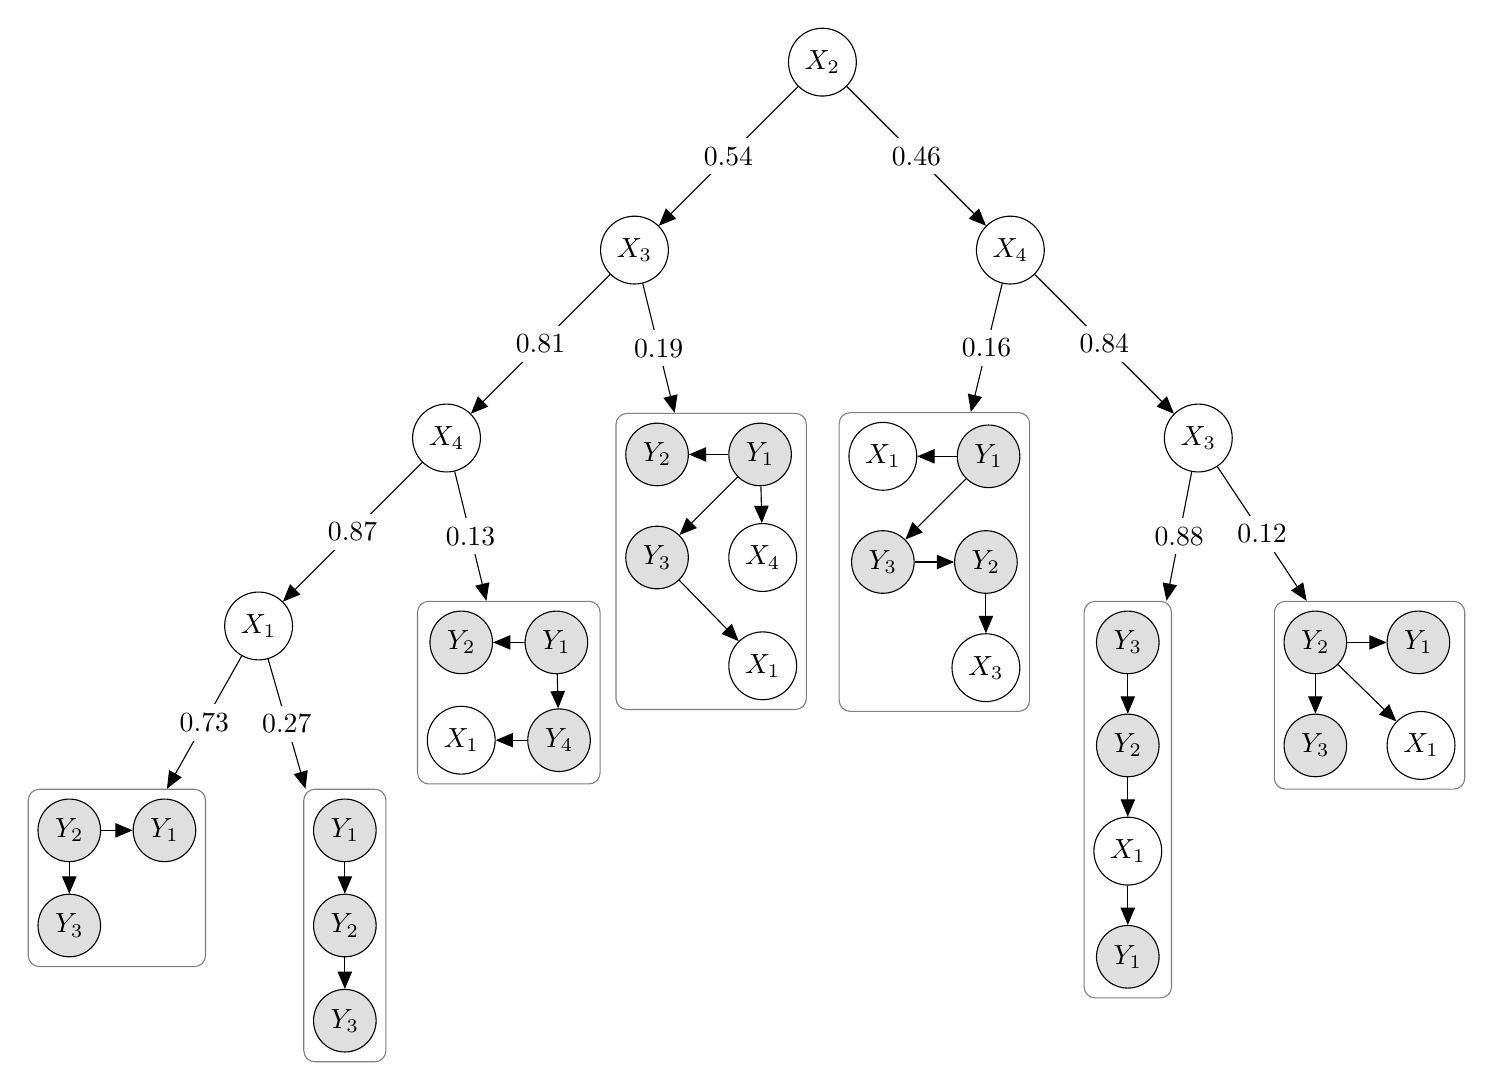
\begin{tikzpicture}
  \node [X] (n1) {$X_2$};    
  \node [X,below left=2.5cm of n1] (n2) {$X_3$};    
  \node [X,below left=2.5cm of n2] (n3) {$X_4$};    
  \node [X,below left=2.5cm of n3] (n4) {$X_1$};    
  \node [X,below right=2.5cm of n1] (n5) {$X_4$};    
  \node [X,below right=2.5cm of n5] (n6) {$X_3$};    

  \node [Y,below right=2cm and 1cm of n2] (n7) {$Y_1$};
  \node [Y,left=0.5cm of n7] (n8) {$Y_2$};
  \node [Y,below=0.5 of n8] (n9) {$Y_3$};
  \node [X,right=0.5 of n9] (n10) {$X_4$};
  \node [X,below=0.5 of n10] (n101) {$X_1$};
  \node [draw=gray,rectangle,rounded corners,fit=(n7) (n8) (n9) (n10) (n101)] (r1) {};
  \draw [->] (n7) -- (n8) ;
  \draw [->] (n7) -- (n9);
  \draw [->] (n7) -- (n10);
  \draw [->] (n9) -- (n101);

  \draw [->] (n2) -- (n3) node [midway,fill=white] {0.81};
  \draw [->] (n2) -- (r1) node [midway,fill=white] {0.19};

  \draw [->] (n1) -- (n2) node [midway,fill=white] {0.54};
  \draw [->] (n1) -- (n5) node [midway,fill=white] {0.46};

  \node [Y,below right=2cm and 0.8cm of n3] (n11) {$Y_1$};
  \node [Y,left=0.4cm of n11] (n12) {$Y_2$};
  \node [X,below=0.4 of n12] (n13) {$X_1$};
  \node [Y,right=0.4 of n13] (n14) {$Y_4$};

  \draw [->] (n11) -- (n12);
  \draw [->] (n14) -- (n13);
  \draw [->] (n11) -- (n14);

  \node [draw=gray,rectangle,rounded corners,fit=(n11) (n12) (n13) (n14)] (r2) {};

  \draw [->] (n3) -- (r2) node [midway,fill=white] {0.13};
  \draw [->] (n3) -- (n4) node [midway,fill=white] {0.87};

  \node [Y,below right=2cm and 0.5cm of n4] (n15) {$Y_1$};
  \node [Y,below=0.4cm of n15] (n16) {$Y_2$};
  \node [Y,below=0.4 of n16] (n17) {$Y_3$};
  \draw [->] (n15) -- (n16);
  \draw [->] (n16) -- (n17);
  \node [draw=gray,rectangle,rounded corners,fit=(n15) (n16) (n17)] (r3) {};

  \node [Y,below left=2cm and 0.6cm of n4] (n19) {$Y_1$};
  \node [Y,left=0.4cm of n19] (n20) {$Y_2$};
  \node [Y,below=0.4 of n20] (n21) {$Y_3$};
  \draw [->] (n20) -- (n19);
  \draw [->] (n20) -- (n21);
  \node [draw=gray,rectangle,rounded corners,fit=(n19) (n20) (n21)] (r4) {};

  \draw [->] (n4) -- (r3) node [midway,fill=white] {0.27};
  \draw [->] (n4) -- (r4) node [midway,fill=white] {0.73};

  \node [Y,below right=2cm and 2.2cm of n6] (n23) {$Y_1$};
  \node [Y,left=0.5cm of n23] (n24) {$Y_2$};
  \node [Y,below=0.5 of n24] (n25) {$Y_3$};
  \node [X,right=0.5 of n25] (n26) {$X_1$};
  \node [draw=gray,rectangle,rounded corners,fit=(n23) (n24) (n25) (n26)] (r5) {};
  \draw [->] (n24) -- (n23);
  \draw [->] (n24) -- (n25);
  \draw [->] (n24) -- (n26);

  \node [Y,below left=2cm and 0.3cm of n6] (n27) {$Y_3$};
  \node [Y,below=0.5cm of n27] (n28) {$Y_2$};
  \node [X,below=0.5 of n28] (n29) {$X_1$};
  \node [Y,below=0.5 of n29] (n30) {$Y_1$};
  \node [draw=gray,rectangle,rounded corners,fit=(n27) (n28) (n29) (n30)] (r6) {};
  \draw [->] (n27) -- (n28);
  \draw [->] (n28) -- (n29);
  \draw [->] (n29) -- (n30);

  \draw [->] (n6) -- (r5) node [midway,fill=white] {0.12};
  \draw [->] (n6) -- (r6) node [midway,fill=white] {0.88};
  \draw [->] (n5) -- (n6) node [midway,fill=white] {0.84};

  \node [X,below left=2cm and 1cm  of n5] (n32) {$X_1$};
  \node [Y,right=0.5 of n32] (n31) {$Y_1$};
  \node [Y,below=0.5 of n32] (n33) {$Y_3$};
  \node [Y,right=0.5 of n33] (n34) {$Y_2$};
  \node [X,below=0.5 of n34] (n35) {$X_3$};
  \draw [->] (n31) -- (n33);
  \draw [->] (n31) -- (n32);
  \draw [->] (n33) -- (n34);
  \draw [->] (n34) -- (n35);
  \node [draw=gray,rectangle,rounded corners,fit=(n31) (n32) (n33) (n34) (n35)] (r7) {};
  \draw [->] (n5) -- (r7) node [midway,fill=white] {0.16};

\end{tikzpicture}
\end{document}
